
\begin{figure}[h]        
        
    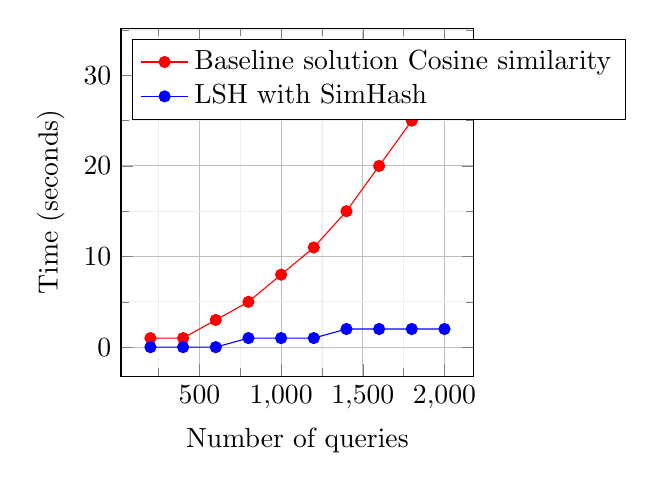
\begin{tikzpicture}
    \begin{axis}[
        xlabel=Number of queries,
        ylabel=Time (seconds),
        height=6cm,
        width = 0.5*\textwidth,
        grid = both,
        minor tick num = 1,
        major grid style = {lightgray},
        minor grid style = {lightgray!25},
        legend cell align = {left},
        legend pos = north west
    ]
    
    % Add values and attributes for the first plot
    \addplot[color=red,mark=*] coordinates {
    	(200, 1)
    	(400, 1)
    	(600, 3)
    	(800, 5)
    	(1000, 8)
    	(1200, 11)
    	(1400, 15)
    	(1600, 20)
    	(1800, 25)
    	(2000, 32)
    };
    
    % Add values and attributes for the second plot
    \addplot[color=blue,mark=*] coordinates {
    	(200, 0)
    	(400, 0)
    	(600, 0)
    	(800, 1)
    	(1000, 1)
    	(1200, 1)
    	(1400, 2)
    	(1600, 2)
    	(1800, 2)
    	(2000, 2)
    };
    
    \legend{Baseline solution Cosine similarity,LSH with SimHash}
    \end{axis}
    \end{tikzpicture}
    
    
    \caption{\normalfont Time performance of the Naive algorithm compared with LSH using SimHash – Variable number of queries}
    \label{fig:lsh_simhash_queries}
\end{figure}
